\section{The Large Hadron Collider}
\label{sec:lhc}
(describe the accelerator complex, proton bunches, c.m. energy, all experiments, run periods, inst. and integrated lumi, Run 3 and HL-LHC plans)

\begin{figure}[H]
  \centering
  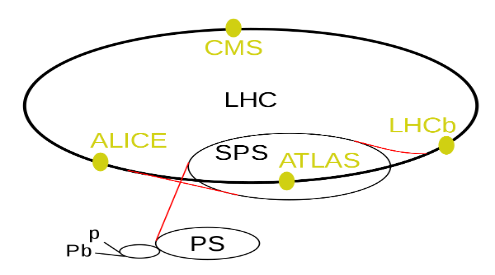
\includegraphics[width=0.7\columnwidth]{./LHCcomplex.png}
  \caption{Diagram of the LHC accelerator complex located in Geneva, Switzerland. Four interaction points are shown for the ALICE, ATLAS
, LHCb, and CMS experiments.}
  \label{fig:LHC}
\end{figure}


\begin{figure}[H]
  \centering
  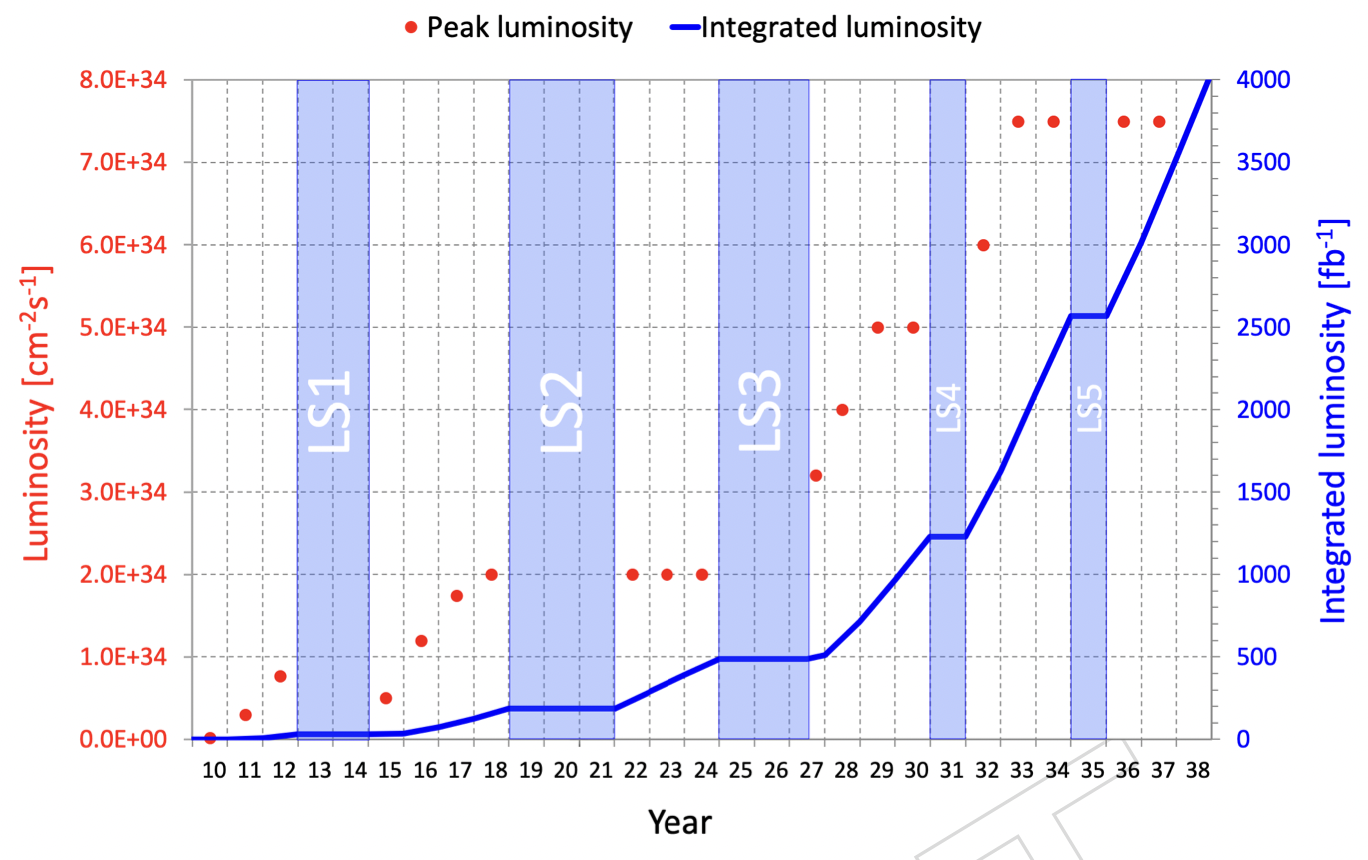
\includegraphics[width=0.8\columnwidth]{./HLLHCLumi.png}
  \caption{Projected performance of the LHC until 2038, which shows the preliminary dates for prolonged stops (LS) of the LHC and lumino
sities. Points show instantaneous luminosity while the line shows luminosity accumulated \cite{collaborations2019report}.}
  \label{fig:LHCPlans}
\end{figure}
